\section{pstree.c}
Trong hệ điều hành xv6, mỗi tiến trình khi sinh ra đều được hệ thống
quản lý thông qua cấu trúc \code{struct proc} nằm trong bảng tiến trình
\code{proc[NPROC]} tại \texttt{kernel/proc.c} \cite{xv6book}. Tuy nhiên,
hệ thống mặc định lại không cung cấp một công cụ hay lời gọi hệ thống
nào để người dùng có thể xem được mối quan hệ phả hệ cha -- con giữa các
tiến trình đang cùng chạy. Để xây dựng được tính năng hiển thị cây tiến
trình tương tự như lệnh \texttt{pstree} trong môi trường Linux, nhóm
cần thiết lập thêm một system call mới với mã định danh \code{SYS\_ptree = 23}
trong tệp \texttt{kernel/syscall.h} \cite{hcmus_os_lab2}.

System call này sẽ nhận vào hai đối số: một con trỏ vùng đệm \code{buf}
trỏ tới mảng cấu trúc và một số nguyên \code{max} đại diện cho số lượng
tiến trình tối đa mà người dùng muốn lấy. Để cả tầng kernel lẫn user
đều có thể hiểu chung một kiểu dữ liệu, nhóm đã định nghĩa cấu trúc
\code{struct ptreeinfo} trong tệp tiêu đề \texttt{kernel/ptree.h} bao
gồm $5$ thông tin cơ bản nhất của một tiến trình: \code{pid} (mã tiến
trình), \code{ppid} (mã tiến trình cha), \code{state} (trạng thái),
\code{memsize} (kích thước bộ nhớ user) và \code{name} (tên tiến trình).

\subsection{Triển khai}
Để triển khai hoàn chỉnh tính năng này, nhóm chia công việc thành hai
phần: xây dựng system call \texttt{ptree} trong kernel để thu thập dữ
liệu an toàn, và viết chương trình \texttt{pstree.c} ở không gian người
dùng (\texttt{user/}) để nhận dữ liệu rồi dựng thành cây hiển thị ra
màn hình.

Đầu tiên, khi người dùng gọi hàm \code{ptree(procs, NPROC)} ở user
space, kernel sẽ tiếp nhận yêu cầu tại hàm \code{sys\_ptree(void)}
trong file \texttt{kernel/sysproc.c}. Tại đây, nhóm sử dụng hai hàm
trợ giúp quen thuộc của xv6 là \code{argaddr(0, \&uaddr)} để lấy địa
chỉ bộ đệm ảo của user và \code{argint(1, \&max)} để lấy số lượng phần
tử tối đa, sau đó chuyển tiếp các tham số này vào hàm xử lý lõi
\code{get\_ptree(uaddr, max)} đặt tại \texttt{kernel/proc.c}.

Khi hiện thực hàm \code{get\_ptree}, kernel cần kiểm tra tính hợp lệ của tham số
và sử dụng khóa để đồng bộ hóa dữ liệu. Đầu tiên, kernel
tiến hành kiểm tra tính hợp lệ của đối số: nếu người dùng truyền vào
\code{max <= 0} hoặc con trỏ rỗng (\code{uaddr == 0}), hệ thống sẽ lập tức
từ chối và trả về $-1$. Kế tiếp, kernel duyệt qua bảng tiến trình
\code{proc[NPROC]}. Vì xv6 vận hành trên môi trường đa lõi (SMP), các tiến
trình khác có thể thay đổi trạng thái liên tục. Do đó, hàm bắt buộc phải gọi
\code{acquire(\&p->lock)} để khóa tiến trình hiện hành trước khi đọc. Nếu tiến
trình chưa được sử dụng (\code{p->state == UNUSED}), ta nhả khóa
\code{release(\&p->lock)} và bỏ qua để chỉ giữ lại các tiến trình thực sự còn sống.

Đối với mỗi tiến trình hợp lệ, kernel trích xuất các thông tin cơ bản bao gồm
\code{pid}, \code{state}, kích thước bộ nhớ \code{p->sz} và tên tiến trình
bằng \code{safestrcpy}. Điểm đặc biệt quan trọng cần lưu ý là khi lấy mã tiến
trình cha (\code{ppid}): tiến trình đầu tiên của hệ thống (\code{initproc})
hoàn toàn không có cha, tức là con trỏ \code{p->parent == 0}. Nếu truy xuất trực
tiếp \code{p->parent->pid} mà không kiểm tra thì sẽ xảy ra lỗi giải tham chiếu
con trỏ rỗng khiến toàn bộ kernel bị sập. Do đó, hệ thống chỉ lấy \code{p->parent->pid}
khi \code{p->parent} tồn tại, ngược lại sẽ gán mặc định bằng $0$.

Sau khi đã nạp đầy đủ thông tin vào biến tạm \code{info}, kernel lập tức gọi
\code{release(\&p->lock)} trước khi tiến hành chuyển dữ liệu ra ngoài. Việc giải
phóng spinlock trước khi gọi \code{copyout} giúp tránh giữ khóa trong thời gian
dài khi truy cập bộ nhớ người dùng, giảm thiểu nguy cơ tắc nghẽn và xung đột khóa.
Vì kernel và user sở hữu hai bảng phân trang hoàn
toàn độc lập (\code{kernel\_pagetable} và \code{p->pagetable}), địa chỉ ảo
\code{uaddr} của user không hề tồn tại trong không gian của kernel. Do đó, ta tuyệt
đối không thể ép kiểu con trỏ C để gán giá trị trực tiếp, mà bắt buộc phải sử
dụng hàm \code{copyout()} của xv6 để kernel tự động tra cứu bảng phân trang của
user và ghi dữ liệu an toàn vào đúng ô nhớ vật lý trong RAM. Vị trí ghi phần tử
thứ \code{count} được tính toán theo độ dời byte: $\text{dst} = \text{uaddr} + \text{count} \times \text{sizeof}(\text{struct } ptreeinfo)$.
Nếu hàm \code{copyout} gặp lỗi (chẳng hạn user truyền địa chỉ ảo ngoài phạm vi cấp phát),
kernel sẽ lập tức dừng lại và trả về $-1$.

\paragraph*{Tái tạo cây và In}: Sau khi kernel đã hoàn tất việc đổ dữ
liệu phẳng về bộ đệm, bước tiếp theo là chương trình \texttt{user/pstree.c}
sẽ dựng lại cây phả hệ cha -- con và in ra màn hình. Để tuân thủ nguyên tắc tách biệt giữa tầng nhân (cung cấp dữ liệu thô) và tầng
người dùng (xử lý định dạng và hiển thị), nhóm lựa chọn thuật toán duyệt theo
chiều sâu (DFS -- Depth-First Search theo thứ tự Pre-order) bằng hàm đệ quy
\code{print\_tree(pid, depth, procs, n)}.
Nhóm quyết định dùng DFS thay vì duyệt theo chiều rộng (BFS -- Breadth-First
Search) bởi vì trên giao diện dòng lệnh vốn chỉ có thể xuất văn bản tuần
tự từ trên xuống, DFS cho phép in ngay tiến trình cha rồi đi sâu vào toàn
bộ các nhánh con cháu của nó trước khi rẽ sang nhánh khác, giúp cấu trúc
thụt lề thể hiện quan hệ cha -- con một cách liền mạch và trực quan nhất.
Ngược lại, nếu dùng BFS (duyệt theo mức), các tiến trình cùng độ sâu sẽ bị
in dàn trải liên tiếp làm đứt gãy mạch phả hệ, đồng thời còn đòi hỏi phải
cài đặt thêm cấu trúc hàng đợi (\texttt{Queue}) phức tạp vốn không có sẵn
trong thư viện xv6. Hơn nữa, DFS đệ quy tận dụng trực tiếp ngăn xếp gọi hàm
(Call Stack) giúp mã nguồn ngắn gọn và không cần cấp phát thêm cấu trúc hàng đợi phụ trợ.

Vì hàm \code{printf} tối giản của xv6 không hỗ trợ định dạng thụt lề
tự động (\code{\%*s}) như thư viện chuẩn của C, nhóm dùng vòng lặp
\code{for} để in ra \code{depth * 2} khoảng trắng tương ứng với độ sâu
của tiến trình trên cây, sau đó in các trường thông tin theo đúng cú
pháp đề bài yêu cầu: \texttt{<pid> <name> state=<state> mem=<memsize>}.
Kế tiếp, hàm sẽ duyệt tìm toàn bộ các tiến trình con có \code{ppid}
bằng với \code{pid} hiện tại và gọi đệ quy tiếp với \code{depth + 1}.
Ở hàm \code{main()}, chương trình tìm các tiến trình gốc không có cha
trong danh sách (\code{has\_parent == 0} hoặc \code{ppid == 0}, tiêu
biểu là \texttt{init}) để phát động hàm đệ quy từ gốc với \code{depth = 0}.
Nhờ đó, cây tiến trình được hiển thị rõ ràng, trực quan và đúng chuẩn quan hệ phân cấp.

\subsection{Kiểm thử}
Sau khi hoàn tất quá trình triển khai system call \texttt{ptree} trong kernel và tiện ích \texttt{pstree} ở user space, nhóm tiến hành thiết lập các kịch bản kiểm thử nhằm kiểm tra tính đúng đắn của giải pháp từ cấu trúc hiển thị phả hệ, mức độ thụt lề cho đến việc xử lý tham số đầu vào (Bảng~\ref{tab:pstree_testcases}).

\begin{table}[htbp]
    \centering
    \small
    \renewcommand{\arraystretch}{1.3}
    \begin{tabularx}{\textwidth}{p{0.36\textwidth} X}
        \toprule
        \textbf{Kịch bản kiểm thử} & \textbf{Mục đích kiểm tra} \\
        \midrule
        \texttt{pstree} (Trực tiếp từ shell) 
            & Kiểm tra hiển thị phả hệ cơ bản của hệ thống gồm tiến trình gốc \texttt{init}, tiến trình dòng lệnh \texttt{sh} và chính tiến trình \texttt{pstree}. \\
        \textbf{Cấu trúc thụt lề phân tầng} 
            & Xác nhận mỗi cấp độ sâu (\texttt{depth}) được thụt lề đúng $2$ khoảng trắng, phản ánh chuẩn xác quan hệ cha -- con phân nhánh từ trên xuống dưới. \\
        \textbf{Tính chính xác của trạng thái} 
            & Kiểm tra trường \code{state}: tiến trình đang thực thi xuất dữ liệu mang trạng thái \code{RUNNING} ($4$), trong khi các tiến trình cha chờ đợi mang trạng thái \code{SLEEPING} ($2$). \\
        \textbf{Xác thực thông tin bộ nhớ} 
            & Xác nhận trường \code{memsize} phản ánh đúng kích thước không gian nhớ của tiến trình (\code{p->sz}). \\
        \textbf{Xử lý tham số biên} 
            & Đảm bảo hàm xử lý tại tầng kernel luôn kiểm tra điều kiện đầu vào, từ chối thực thi và trả về mã lỗi $-1$ an toàn khi người dùng truyền \code{max <= 0} hoặc con trỏ bộ đệm rỗng (\code{uaddr == 0}). \\
        \bottomrule
    \end{tabularx}
    \caption{Các kịch bản kiểm thử tính năng hiển thị cây tiến trình}
    \label{tab:pstree_testcases}
\end{table}

Kết quả thực nghiệm trên môi trường giả lập QEMU (Hình~\ref{fig:pstree_result}) cho thấy chương trình hoạt động đúng theo đặc tả của bài thực hành:
\begin{itemize}[noitemsep, topsep=2pt]
    \item \textbf{Cấu trúc phả hệ phân tầng (Hình~\ref{fig:pstree_result}):} Cây tiến trình được dựng và in ra màn hình tuần tự với gốc là \texttt{init} (PID $1$, $\text{depth} = 0$). Tiến trình con \texttt{sh} (PID $2$, $\text{depth} = 1$) được thụt lề $2$ khoảng trắng, và tiến trình cháu \texttt{pstree} (PID $5$, $\text{depth} = 2$) do shell khởi sinh được thụt lề $4$ khoảng trắng, thể hiện rõ ràng quan hệ phả hệ qua $3$ thế hệ tiến trình.
    \item \textbf{Tính chính xác của dữ liệu và trạng thái:} Tất cả các thuộc tính bao gồm \code{pid}, tên tiến trình, trạng thái (\code{RUNNING} cho \texttt{pstree} và \code{SLEEPING} cho các tiến trình cha), cùng kích thước bộ nhớ (\code{mem=20480} và \code{mem=24576}) đều được kernel thu thập nhất quán và truyền an toàn ra không gian người dùng.
\end{itemize}

\begin{figure}[H]
    \centering
    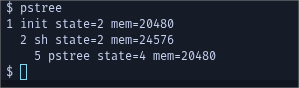
\includegraphics[width=0.62\textwidth]{images/pstree.png}
    \caption{Ảnh chụp kết quả thực thi lệnh \texttt{pstree} trên môi trường QEMU}
    \label{fig:pstree_result}
\end{figure}
